% Setup
\documentclass[a4 paper, 12pt]{article}

% Title
\title{COSC3000 - COMPUTER GRAPHICS REPORT \\ --- \\Olympics Athletic Track}
\author{Tean-louise Cunningham (42637460)}
\date{\today}

% Margins
\usepackage{geometry}
\geometry{margin=2cm}

% Images
\usepackage{graphicx}
\usepackage{float}
\usepackage[export]{adjustbox}
\setlength{\intextsep}{5pt plus 2pt minus 2pt}
\usepackage[font=small,skip=5pt]{caption}


% Paragraph
\setlength{\parindent}{2em}
\setlength{\parskip}{1em}

% Text Formatting
\usepackage[utf8]{inputenc}
\usepackage[english]{babel}

% List spacing
\usepackage{enumitem}
\setlist{noitemsep, topsep=0pt}
\setlist[enumerate]{parsep=5pt} 

% Text Color
\usepackage{xcolor}

% Hyperlinks
\usepackage{hyperref}
\hypersetup{
    colorlinks=true,
    linkcolor=black,
    filecolor=black,      
    urlcolor=blue,
}

% Appendix
\usepackage{appendix}

% Include pdf
\usepackage{standalone}
\usepackage{pdfpages}

% Borders
\usepackage{mdframed}

% Appendix
\usepackage{appendix}

\usepackage{listings}


%%%%%%%%%%%%%%%%%%%%%%%%%%%%%%%%%%%%%%%%%%
% DOCUMENT
\begin{document}

% Title
\maketitle
    \begin{figure} [H]
        \centering
        \includegraphics[width=0.95\textwidth]
            {./images/title.png}                  
    \end{figure}  


% Table of contents
\pagebreak
\tableofcontents
\pagebreak
\listoffigures

% INTRODUCTION
\pagebreak
\section{Introduction}
In continuance of the exploration of the Olympics from the visualisation project, a graphic simulation of running on an athletic track will be simulated. The main stadium of an Olympics is the most integral location as it hosts the opening and closing ceremonies, the lighting of the touch and the most popular events. The architecture and design choices of these stadiums ensure athletes can compete in optimal circumstances and thousands of spectators can experience these feats. This project will highlight the ingenuity of these stadiums by offering the opportunity to view its design in detail as a competitor on its athletic track. This will be achieved using the provided mega\_racer files, demo and instructions as a base, and the Tokyo National Stadium, which is set to host the 2020 Olympics as inspiration.

% MEGA RACER
\section{Mega Racer - Tier 1}

%% 1.1
\subsection{1.1 - Scale the terrain grid}
In terrain.py load() change zPos from 0 to the below to set the height of the terrain. Also, the last line from racer.py was uncommented so the racer can follow the height.   
    \begin{lstlisting}[language=python]
# terrain.py
def load(...):
    ...
    zPos = red * self.heightScale
    \end{lstlisting}

The height of the terrain is indicated by the shading of red in the provided track image and heightScale refers to appropriate height to x and y measurements given. 
    \begin{figure} [H]
        \centering
        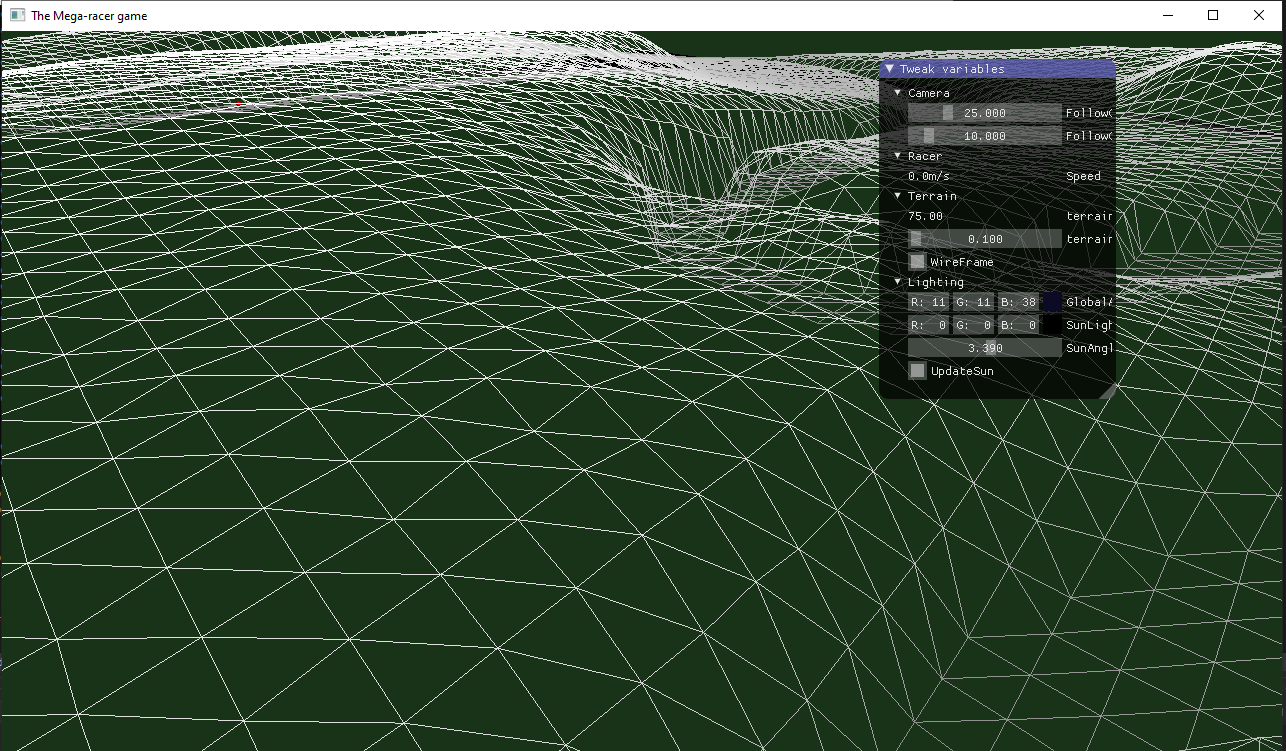
\includegraphics[width=0.8\textwidth, frame]
            {./images/1.1.PNG}
        \caption{1.1}
    \end{figure}  
   

%% 1.2
\subsection{1.2 - Set up a camera to follow the racer}
To start I looked at the code to understand what was happening and what each of the variables related to, particularly g\_viewPosition, g\_viewTarget and g\_viewUp. I found they were being called in mega\_racer.py in \textit{renderFrame()}:
    \begin{lstlisting}[language=python]
# mega_racer.py 
def renderFrame(...):
    ...
    view.worldToViewTransform = lu.make_lookAt(g_viewPosition, 
                                                g_viewTarget, 
                                                g_viewUp)
    \end{lstlisting}

Then I headed to \textit{make\_lookAt()} to see the functionality of the function and parameters that the arguments were being used for. The function makes a transformation from world to view space inversely by calling another function \textit{make\_lookFrom()} with a modified target parameter for smooth movement.  
    \begin{lstlisting}[language=python]
# lab_utils.py
def make_lookAt(eye, target, up):
    return make_lookFrom(eye, 
                        np.array(target[:3]) - np.array(eye[:3]), 
                        up)
    --> 
def make_lookFrom(eye, direction, up):
    .....
    \end{lstlisting}

Also, the examples from lab2 use similar functions in the same manner:
    \begin{lstlisting}[language=python]
# Lab 2 (1) - Q5
worldToViewTransform = magic.make_lookAt(eyePos, [0,0,0], [0,1,0])
# Lab 2 (2) 
worldToViewTransform = magic.make_lookFrom(g_cameraPosition,   
                                            cameraDirection, 
                                            [0,1,0])
    \end{lstlisting}
    
Therefore, the variables have the following meanings:
    \begin{itemize}
        \item g\_viewPosition = eye (location of camera, camera position)
        \item g\_viewTarget = target (point to aim, camera direction=target-eye)
        \item g\_viewUp = up (rough up direction)
    \end{itemize}    
    
With this understanding I could start to assign these variables appropriately to get the camera in the correct position. Firstly, it was clear that the 'target' needed to be updated to the position of the racer as this where the camera needs to be pointing. 
    \begin{lstlisting}[language=python]
# mega_racer.py
def update(...):
    ...
    g_viewTarget = g_racer.position
    \end{lstlisting}

Secondly, the position of the camera needed to be updated to take into account corresponding position of the racer for all coordinates. According to .... the 'desiredPosition = target.position + offset'. Thirdly, all coordinates of the of the camera needed to include the follow offset to be behind and above the racer. Additionally, the z coordinates needed to take into account the look offset of the camera as this is how it is looking at it from above.
    \begin{lstlisting}[language=python]
# mega_racer.py
def update(...):
    ...
    for i in range(0,3):
        g_viewPosition[i] = g_racer.position[i] 
                            + g_followCamOffset
    g_viewPosition[2] += g_followCamLookOffset
    \end{lstlisting}

After running these changes I could see that the camera was almost right, however it wasn't facing the correct direction; directly behind the racer. 
    \begin{figure} [H]
        \centering
        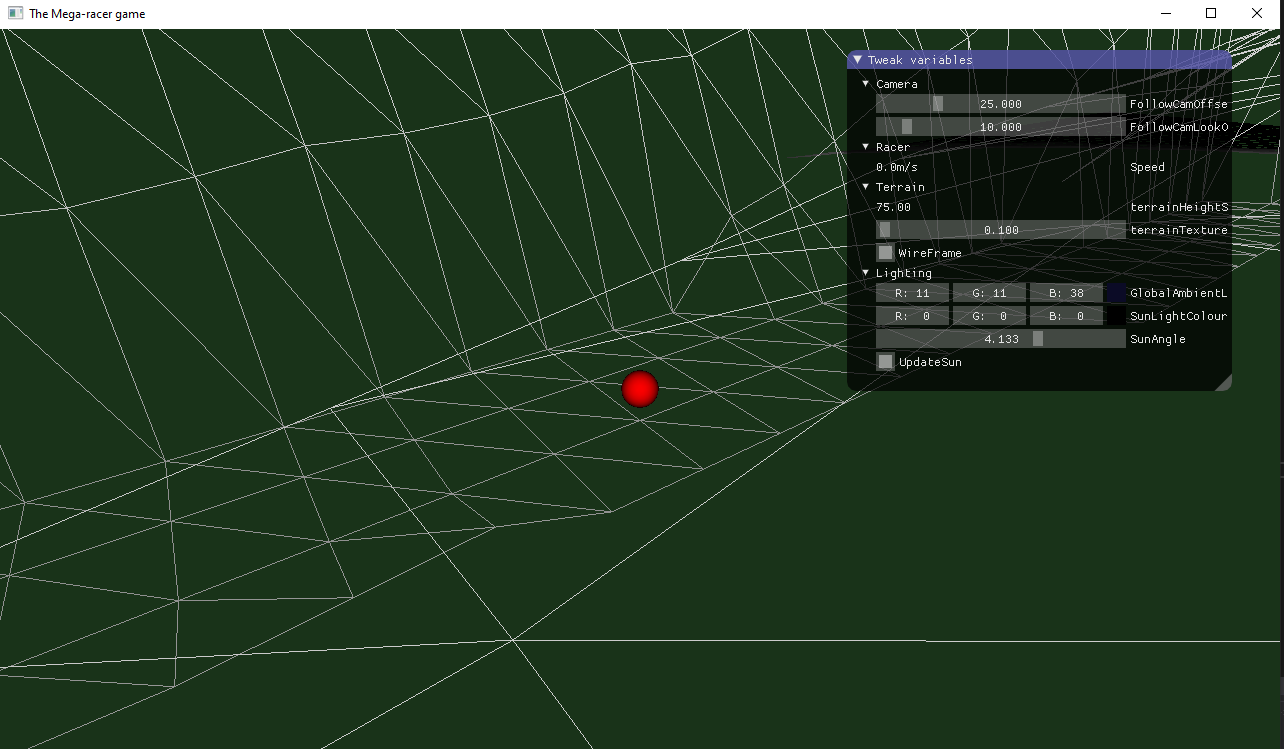
\includegraphics[width=0.8\textwidth, frame]
            {./images/1.2_a.PNG}
        \caption{1.2 - First Attempt}
    \end{figure}

On closer inspection of the Racer class I identified a variable called heading which controlled the direction of the racer. Since the camera needed to be behind the racer, the view position had to be multiplied by the inverse of the racer direction.
    \begin{lstlisting}[language=python]
# mega_racer.py
def update(...):
    ...        
    for i in range(0,3):
        g_viewPosition[i] = g_racer.position[i] 
                            + g_followCamOffset 
                            * -g_racer.heading[i]
    g_viewPosition[2] += g_followCamLookOffset
    \end{lstlisting}

This produced the correct result! The camera was now the position of the racer with the offsets applied at the appropriate direction to the racer's movement.
    \begin{figure} [H]
        \centering
        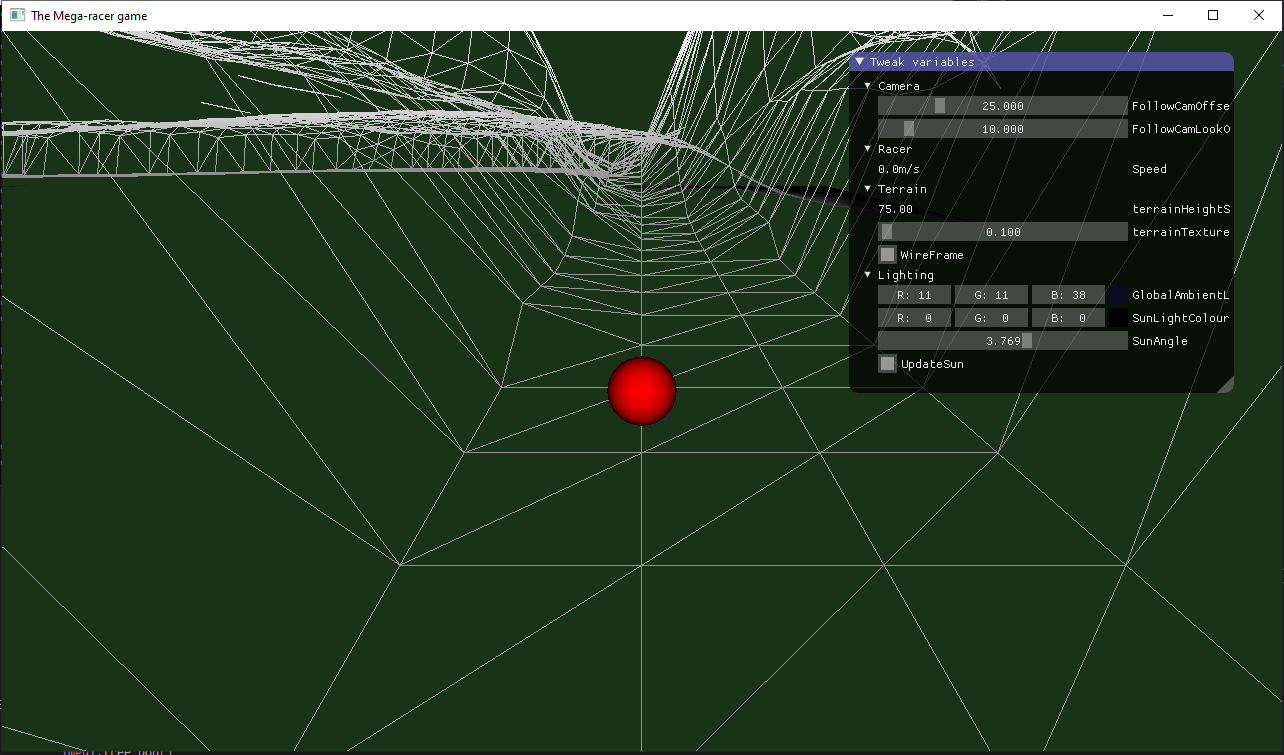
\includegraphics[width=0.8\textwidth, frame]
            {./images/1.2_b.PNG}
        \caption{1.2 - Final Attempt}
    \end{figure}  

%% 1.3
\subsection{1.3 - Place and orient a model for the racer}
Looking at the comments in the code I found two places with TODO for this section in racer.py; render() and load(). Starting with rendering the model I look at mega\_racer.py to see how this function was being called. The racer was being rendered in renderFrame().
    \begin{lstlisting}[language=python]    
# mega_racer.py
def renderFrame(...):
    ...
    g_racer.render(view, g_renderingSystem)  
-->
#racer.py - Racer
def render(self, view, renderingSystem):
    .....
    \end{lstlisting}  

The the view is of ViewParams class and is set up to project and transform from view to clip space, and world to view space. The renderingSystem parameter is of RenderingSystem class. The task for render() is to draw the model and this class has the drawObjModel() function mentioned in the project notes that needs to be used. This function call is added to Racer.render(). In the Racer class there is model variable set to None, and view is passed in as an argument to render(). The only missing parameter is the modelToWorldTransform.
    \begin{lstlisting}[language=python]   
# mega_racer.py - RenderingSystem
def drawObjModel(self, model, modelToWorldTransform, view):
    ...
        -->
# racer.py - Racer
def render(self, view, renderingSystem):
    renderingSystem.drawObjModel(self.model, ???, view)
    \end{lstlisting}  

The project notes mention make\_mat4\_from\_zAxis() as a useful function for transforming the model to the world. This function is in the lab\_utils file (imported as lu in racer.py). The function takes the parameters translation, zAxis and yAxis. The zAxis represents forwards and the yAxis represents up. Therefore, for this world, the z an y axis will act conventionally to the same. This means that the z-axis is the same as the direction of the racer (the heading) and the y-axis is equal to up view of the racer as determined by g\_viewUp in mega\_racer.py. The translation parameter refers to the position of model after all the relevant modifications to the coordinates, in this case that is the position of the racer.
    \begin{lstlisting}[language=python]  
#lab_utils.py    
def make_mat4_from_zAxis(translation, zAxis, yAxis):
    ...
-->
# racer.py - Racer
def render(...):
    modelToWorldTransform = lu.make_mat4_from_zAxis(self.position, 
                                                    self.heading, 
                                                    [ 0.0, 0.0, 1.0 ])
    \end{lstlisting}

After running this code, there was an error message relating to the model; it is of none type. So the next step is to create and load the racer model in load(). 
    \begin{figure} [H]
        \centering
        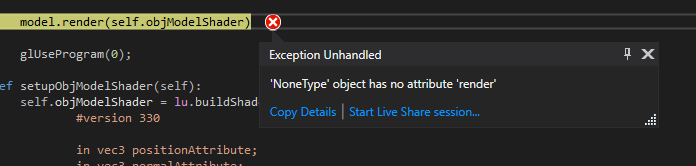
\includegraphics[width=0.8\textwidth, frame]
            {./images/1.3_a.PNG}
        \caption{1.3 -Error}
    \end{figure}

Looking at mega\_racer.py the load() method is called with three parameters; the object file for the racer, the terrain and the rendering system. The purpose of the load() function is to create and load the model. 
    \begin{lstlisting}[language=python]
# mega_racer.py
g_racer.load("data/racer_02.obj", g_terrain, g_renderingSystem)
-->
# racer.py - Racer
def load(self, objModelName, terrain, renderingSystem):
        .....    
    \end{lstlisting}

The rendering system there seemed to be no relevant functions. In the project notes there was mention that the Racer class relied on the ObjModel class, and since drawObjModel() draws ObjModel's then the racer model needed to be an instance of this class. Looking at ObjModel\_\_init\_\_() the only requirement argument is the filename which is given.
    \begin{lstlisting}[language=python]
    self.model = ObjModel(objModelName)
    \end{lstlisting}   

Now the model for the racer has replaced the red dot and the movement relating to the arrows in accurate.
\begin{figure} [H]
    \centering
    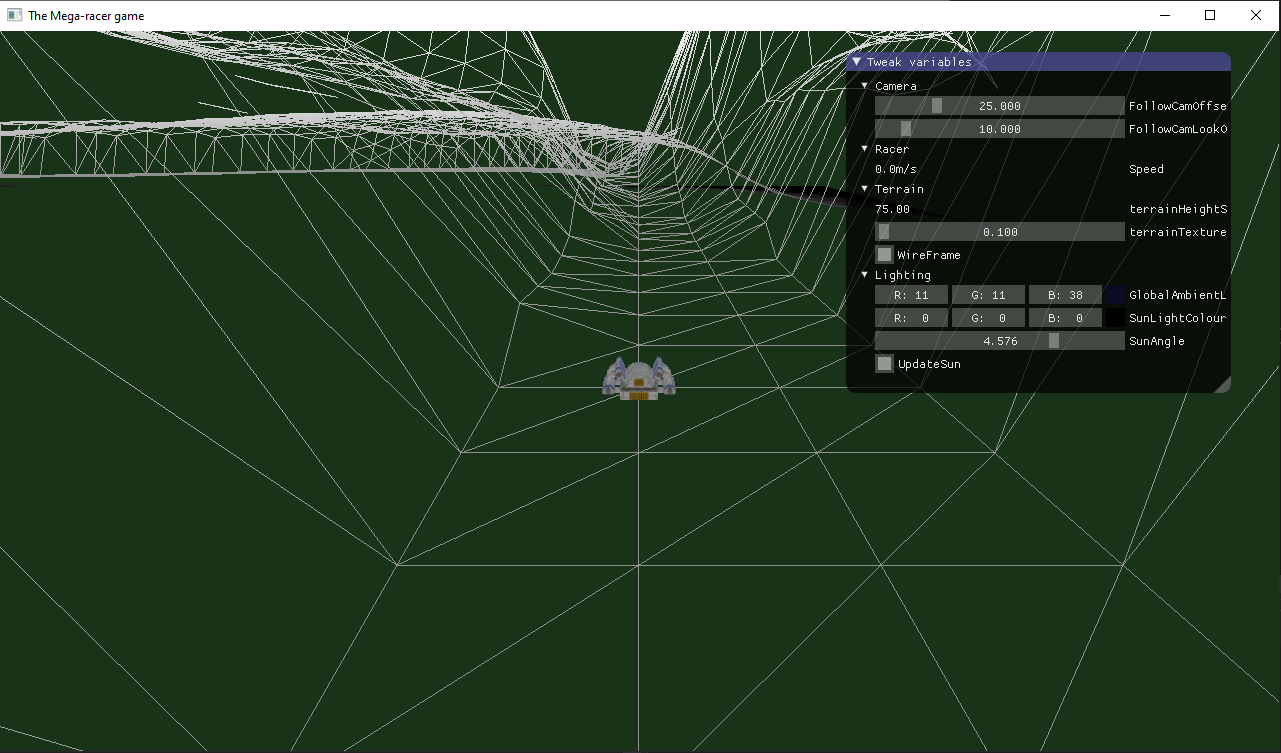
\includegraphics[width=0.8\textwidth, frame]
        {./images/1.3_b.PNG}
    \caption{1.3 - Final}
\end{figure}

%% 1.4
\subsection{1.4 - Texture the terrain}
There are three steps to complete this section in terrain.py. 

\textbf{(1) render() - need to bind the grass texture to the right texture unit.} \\ 
The hint is to is to use lu.bindTexture. This function, bindTexture(), takes two arguments texUnit and textureId. A similar function is used in lab\_utils.py (Lab Code, 2020), also called bindTexture(). In order to use the bindTexture in render() for the project I looked at how it was called in lab 5 question 12 (Lab Code, 2020).
    
    \begin{lstlisting}[language=python]
# Lab - lab_utils.py 
def bindTexture(texUnit, textureId, textureType = GL_TEXTURE_2D):
    ...
    -->
# Lab 5 Q12 - lab_5_template_2.py
g_detailTexture = None
def renderFrame(...):
    .....
    lu.bindTexture(0, g_detailTexture)
    lu.setUniform(g_shaderProgram, "baseTexture", 0)
    \end{lstlisting}

The textureId was first declared and then passed in and the texUnit set to 0. In terrain.py the texUnit is given as TU\_Grass (also equal to 0) and the textureID needs to be declared. Additionally, setUniform() needs to be called to set the shader. Updating the variable names the same was added to terrain.py.
    \begin{lstlisting}[language=python]       
# terrain.py
grassTexture = None

def render(...):
    ....
    lu.bindTexture(self.TU_Grass, self.grassTexture)
    lu.setUniform(self.shader, "grassTexture", self.TU_Grass)        
    \end{lstlisting}

   
\textbf{(2) load(): Compute the texture coordinates and sample the texture for the grass and use as material colour.} \\
As per the project notes the variable textureXyScale is to be used to scale the texture coordinates and is already set to a factor of 0.1 so the texture repeats every 10 metres. Also the world space coordinates should be used  to sample the texture in the fragment shader. To determine how to set the sample I looked at Lab 5 question 12 which sets the colours of the texture in the fragment shader.
\begin{lstlisting}[language=python] 
# Lab 5 - Q12   
def initResources():
    .....         
    in vec2 v2f_textureCoord;
    uniform sampler2D detailTexture; 
    uniform float texCoordScale; 
    out vec4 fragmentColor;
    void main() 
    {...
        vec3 detailColour = texture(detailTexture, 
                            v2f_textureCoord * texCoordScale).xyz;      
        fragmentColor = vec4(detailColour, 1.0);
    }        
\end{lstlisting}

From this example it is evident that the three arguments for texture() need to be assigned to the new materialColour (i.e. detailColour).
    \begin{itemize}
        \item detailTexture: The grass colour is similar to the detailColour so the detailTexture is equivalent to the grassTexture.
        \item texCoordScale: In lab 5 the v2f\_textureCoord is a 2 dimensional out vector from the vertex shader. As per the project notes, since the vertex is regular, we can replicate this same behaviour by only selecting the x and y coordinates of the world space which are stored in v2f\_worldSpacePosition.
        \item v2f\_textureCoord: The textCoordScale in lab 5 is a new name for the given g\_texCoordScale which is declared and uniformly set for the shader as texCoordScale. The same is done for textureXyScale in Terrain which as mentioned is nominated in the project notes as the scale for the texture coordinates.    
    \begin{lstlisting}[language=python] 
# Lab 5 
g_texCoordScale = 7.0
def renderFrame():
    .....
    lu.setUniform(g_shaderProgram, "texCoordScale", g_texCoordScale)

# terrain.py
textureXyScale = 0.1
def render():
    lu.setUniform(self.shader, 
                    "terrainTextureXyScale", 
                    self.textureXyScale);
    \end{lstlisting}
    \end{itemize}

Putting this all together we get the following code to calculate the coordinates and sample the texture for the grass, overriding the existing material colour.
    \begin{lstlisting}[language=python] 
# terrain.py - Terrain
def load(...):
    ...
    fragmentShader =
        ...
        void main()
        {
            vec3 grassColour = texture(grassTexture, 
                                        v2f_worldSpacePosition.xy 
                                            * terrainTextureXyScale).xyz;
            materialColour = grassColour;
            ...
        }
    \end{lstlisting}

\textbf{(3) load() - fragmentShader: Load texture and configure the sampler.} \\
Also in lab 5, in initResources() after declaring the shader the image is opened and the texture is mapped (glTextParameter), then the texture is loaded using lu.loadTexture(). A similar function can be found in the ObjModel.py (instead of lab\_utils.py) and performs the same actions. It also sets the texture to wrap repeatedly as desired.
    \begin{lstlisting}[language=python]   
# Lab 5 
g_detailTexture = lu.loadTexture("data/details.jpg");
--> 
def loadTexture(fileName): 
    ....

# ObjModel.py - ObjModel
def loadTexture(self, fileName, basePath, srgb):
    ......
    glTexParameteri(GL_TEXTURE_2D, GL_TEXTURE_WRAP_S, GL_REPEAT);
    glTexParameteri(GL_TEXTURE_2D, GL_TEXTURE_WRAP_T, GL_REPEAT);
    \end{lstlisting}

To load the texture for the terrain this function needs to be called with the relevant parameters.
    \begin{lstlisting}[language=python]   
# terrain.py - Terrain
def load(...):
    self.grassTexture = ObjModel.loadTexture("grass2.png", "data", True)
    \end{lstlisting}

\begin{figure} [H]
    \centering
    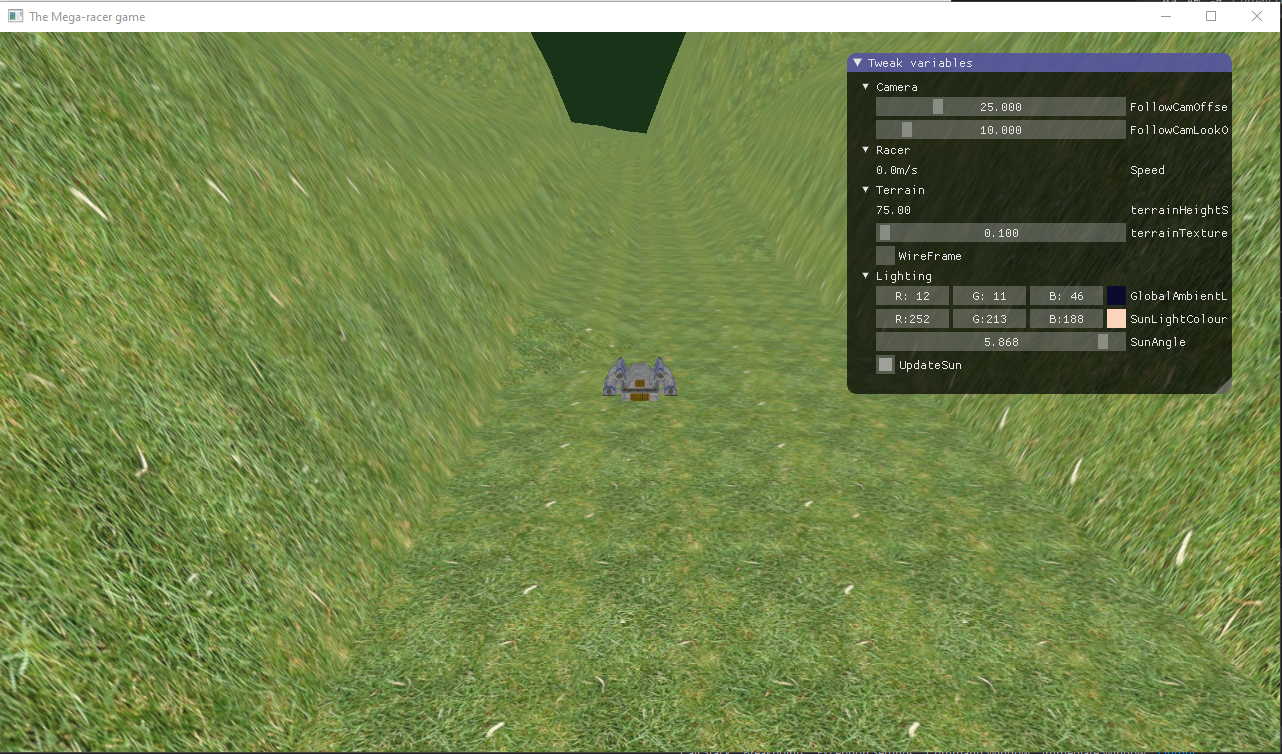
\includegraphics[width=0.8\textwidth, frame]
        {./images/1.4.PNG}
    \caption{1.4 - Final}
\end{figure}



\subsection{1.5 Lighting from the sun}  

The project notes explain that the code for the light should be added to the computeShading() function in RenderingSystem class as part of the commonFragmentShaderCode variable. This function is called in setUpModelShader() where the viewSpaceNormal and viewSpacePosition variables are declared by the vertex shader, materialColour is declared as materialDiffuse in the fragment shader, and viewSpaceLightPosition and sunLightColour are carried over from the commonShaderCode variable. 
    \begin{lstlisting}[language=python] 
#  mega_racer.py - RenderingSystem
def setupObjModelShader(...):
    v2f_viewSpaceNormal = normalize(modelToViewNormalTransform * normalAttribute);
    v2f_viewSpacePosition = (modelToViewTransform * vec4(positionAttribute, 1.0)).xyz;
    .....
    vec3 materialDiffuse = texture(diffuse_texture, 
                                    v2f_texCoord).xyz 
                                    * material_diffuse_color;
    vec3 reflectedLight = computeShading(materialDiffuse, 
                                            v2f_viewSpacePosition, v2f_viewSpaceNormal, viewSpaceLightPosition, 
                                            sunLightColour
                                        ) + material_emissive_color;
    \end{lstlisting}

A couple of things to keep in mind:
    \begin{itemize}
        \item position of sun = g\_sunPosition: The sun is set to move around around the world.
        \item colour of sunlight = g\_sunLightColour = lightColour
        \item all parameters om shading must be the same space -> set as view space (same as lab 4) 
        \item sun is defined in world space
        \item The computeShading function needs to be called from each function -> this is already done.
        \item Need to make sure don't just have Lambertian term -> Fixed by multiplying by materialDiffuse term.
        \item Use clamping to check when light is behind surface
    \end{itemize}


To create the lighting effect required, all of the code followed that of fragmentShader.glsl in Lab 4. Question 1 was already provided as a basic shader. The view space is used for shading calculations. The computeShading() function is setup with five parameters, all of which are used to return a light value.
    \begin{lstlisting}[language=python] 
# mega_racer.py - RenderingSystem
commonFragmentShaderCode =
    ...
    vec3 computeShading(vec3 materialColour, 
                        vec3 viewSpacePosition, 
                        vec3 viewSpaceNormal, 
                        vec3 viewSpaceLightPos, 
                        vec3 lightColour)
    {
        return lightValue;
    }
    \end{lstlisting}

\textbf{(1) The direction towards the source of the light.} \\
Starting from Lab 4, question 2, the first step is to compute the normalised direction towards the light from the shading point in view space. The light position is stored as viewSpaceLightPosition and the current point is viewSpacePosition (provided by the vertex shader). 
    \begin{lstlisting}[language=python] 
# Lab 4 - Q2 - FragmentShader
vec3 viewSpaceDirToLight = normalize(viewSpaceLightPosition - viewSpacePosition);
    
# mega_racer.py - RenderingSystem
commonFragmentShaderCode =
    ...
    vec3 computeShading(...)
    {
        vec3 viewSpaceDirToLight = normalize(viewSpaceLightPos- viewSpacePosition);
        return viewSpaceDirToLight;
    }
    \end{lstlisting}

    \begin{figure} [H]
        \centering
        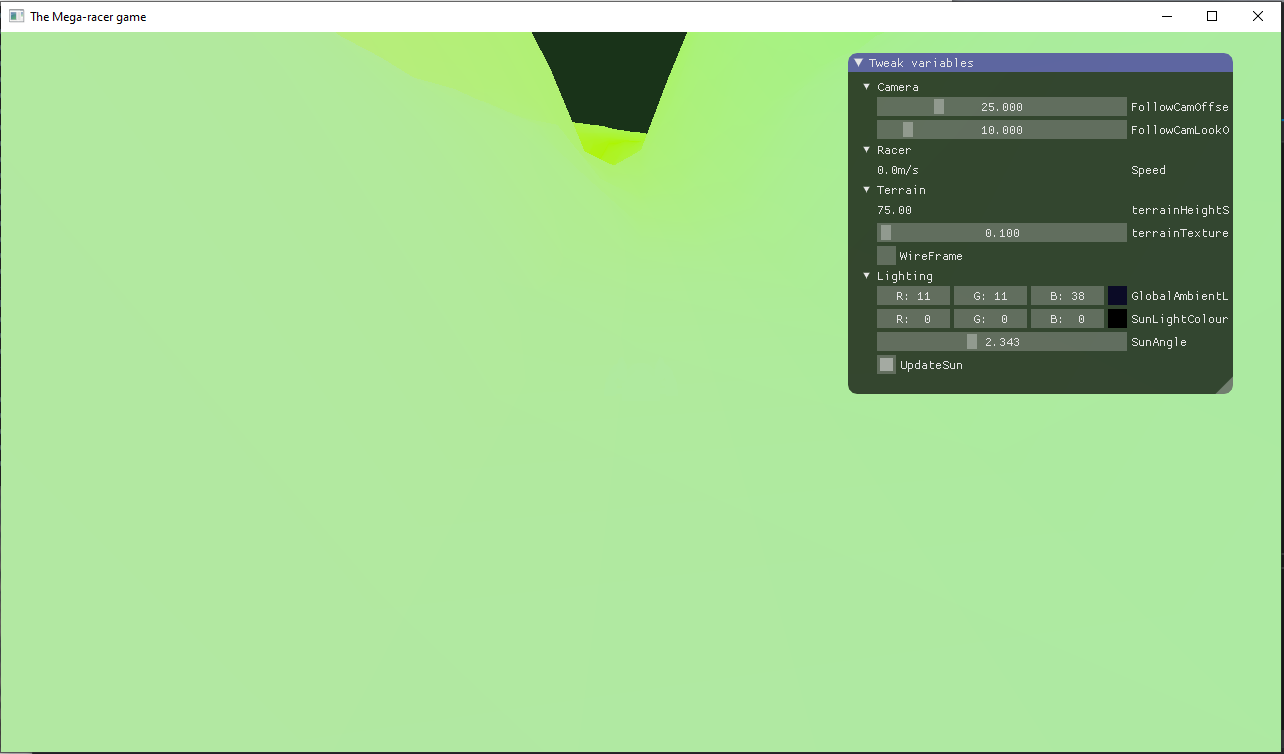
\includegraphics[width=0.8\textwidth, frame]
            {./images/1.5_a.PNG}
        \caption{1.5 - Step 1}
    \end{figure}

\textbf{(2) Compute the incoming light intensity.}
Use the calculated direction to calculate the incoming light intensity. As mentioned, in mega\_racer.py three variable of viewSpaceNormal is already provided by the vertex shader. This maintains the unit-length property of the normal.
    \begin{lstlisting}[language=python] 
# Lab 4 - Q2 - FragmentShader
vec3 viewSpaceNormal = normalize(v2f_viewSpaceNormal);
float incomingIntensity = max(0.0, dot(viewSpaceNormal, viewSpaceDirToLight));

# mega_racer.py - RenderingSystem
commonFragmentShaderCode =
    ...
    vec3 computeShading(...)
    {
        ...
        float incomingIntensity = max(0.0, dot(viewSpaceNormal, viewSpaceDirToLight));
        return incomingIntensity;
    }
    \end{lstlisting}

    \begin{figure} [H]
        \centering
        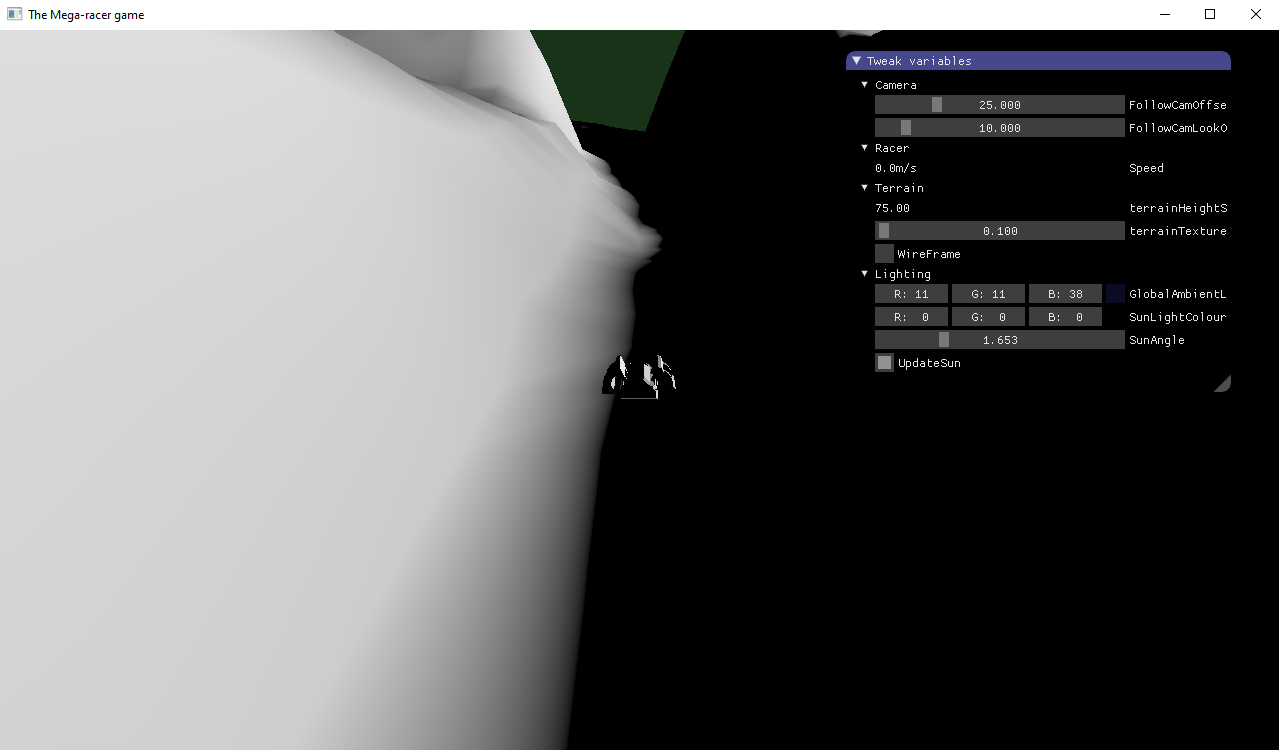
\includegraphics[width=0.8\textwidth, frame]
            {./images/1.5_b.PNG}
        \caption{1.5 - Step 2}
    \end{figure}


\textbf{(3) Modify the light that is emitted by the light source to have the correct colour and maximum intensity.}
This fixes the proportion if incoming light arriving at the surface so it is the correct colour and maximum intensity
    \begin{lstlisting}[language=python] 
# Lab 4 - Q2 - FragmentShader
vec3 incomingLight = incomingIntensity * lightColourAndIntensity;

# mega_racer.py - RenderingSystem
commonFragmentShaderCode =
    ...
    vec3 computeShading(...)
    {
        ...
        vec3 incomingLight = incomingIntensity * lightColour;
        return incomingLight;
    }        
    \end{lstlisting}

    \begin{figure} [H]
        \centering
        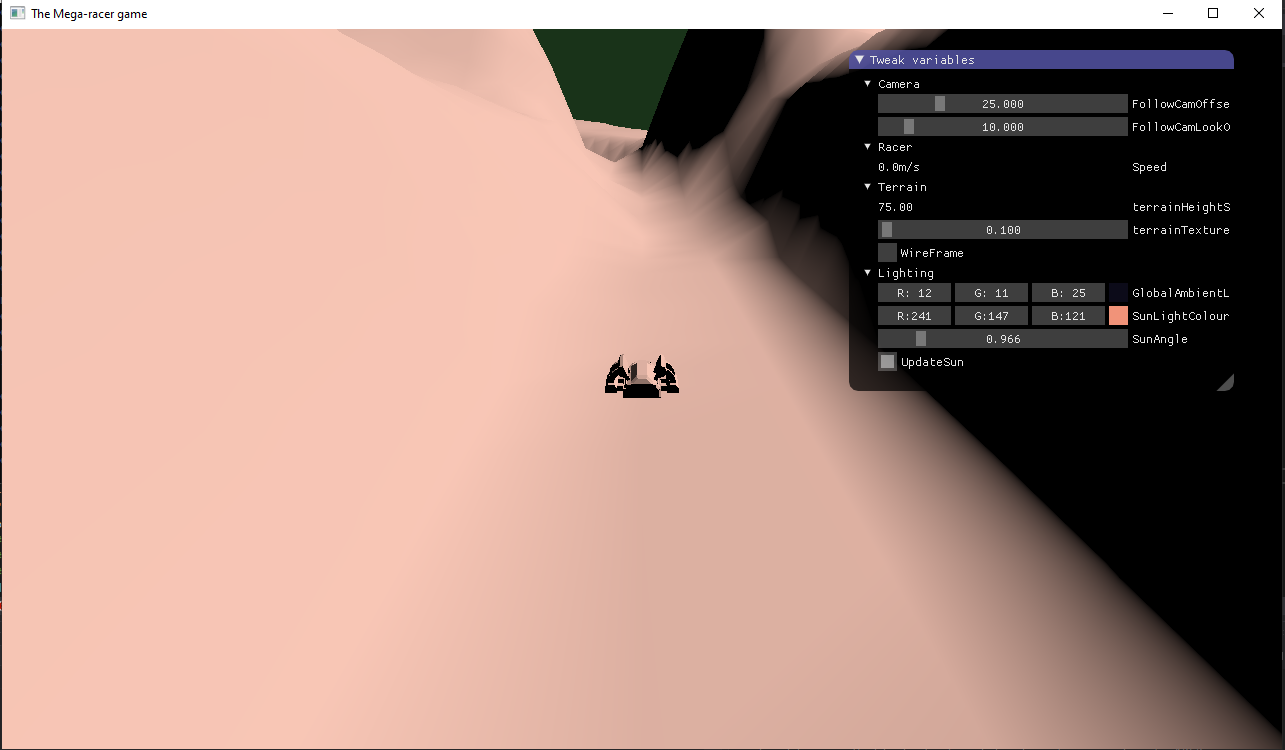
\includegraphics[width=0.8\textwidth, frame]
            {./images/1.5_c.PNG}
        \caption{1.5 - Step 3}
    \end{figure}


\textbf{(4) Diffuse Lambertian Reflection.}
Moving on to question 3 of lab 4, the next step is to diffuse the Lambertian reflection by multiplying the incoming light with a constant that represents the reflection of the material for the given spectrum. The argument passed as materialColour should provide this representation, as provided by the materialDiffuse variable passed in to computeShading() in setUpObModelShader(). This variable follows the same pattern as that of lab 4.  
    \begin{lstlisting}[language=python] 
# Lab 4  - FragmentShader
vec3 materialDiffuse = texture(diffuse_texture, v2f_texCoord).xyz * material_diffuse_color;
vec3 outgoingLight = incomingLight * materialDiffuse;

# mega_racer.py - RenderingSystem
commonFragmentShaderCode =
    ...
    vec3 computeShading(...)
    {
        ...
        vec3 outgoingLight = incomingLight * materialColour;
        return outgoingLight;
    }                            
    \end{lstlisting}

    \begin{figure} [H]
        \makebox[\textwidth]{%
        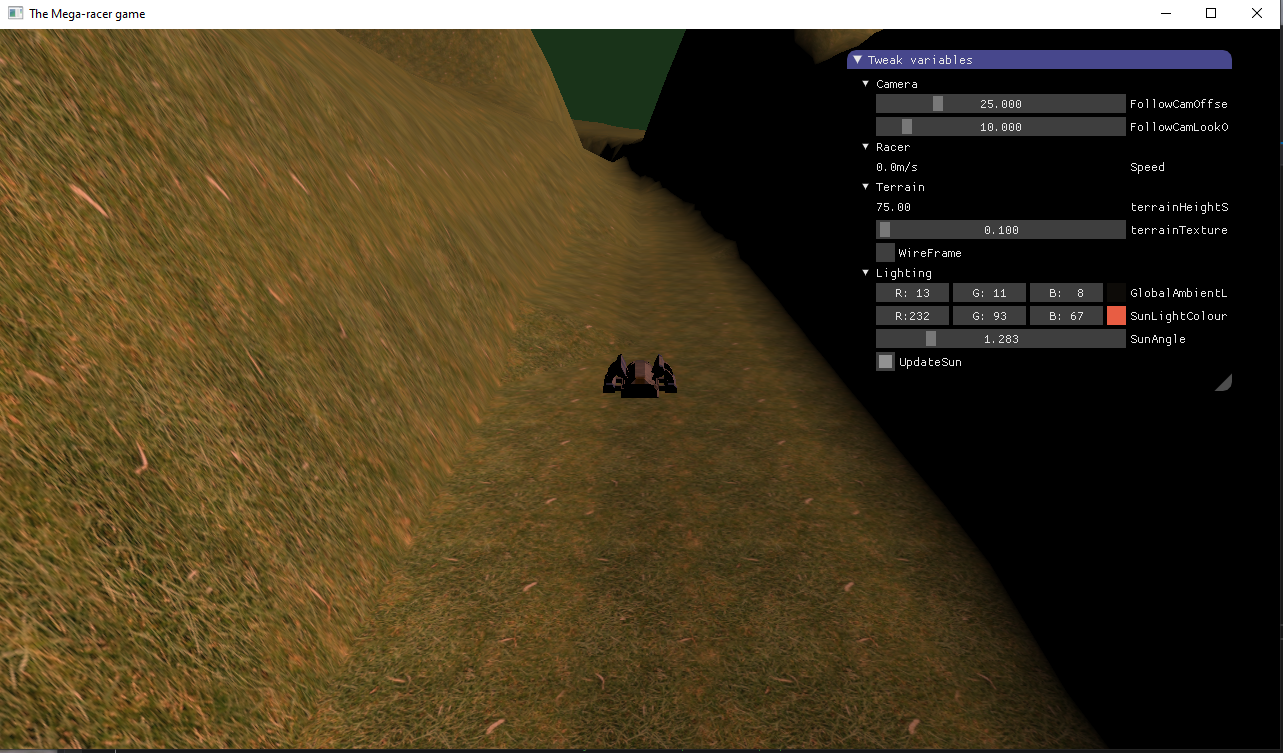
\includegraphics[width=0.49\textwidth, frame]
            {./images/1.5_d_1.PNG}%
        \hfill
        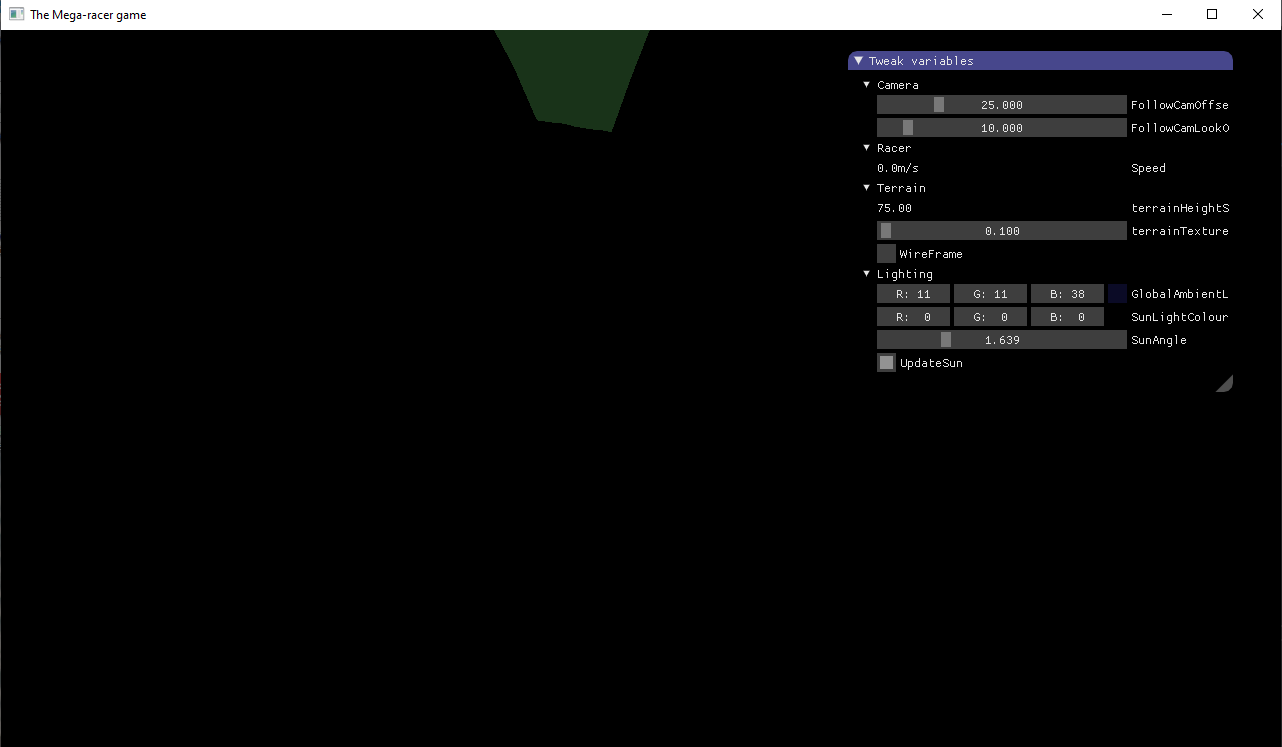
\includegraphics[width=0.49\textwidth, frame]
            {./images/1.5_d_2.PNG}
        }        
        \caption{1.5 - Step 5}   4
    \end{figure}

\textbf{(5) Take into account the indirect light.}
The next step is to handle the ambient light. This step builds on step 3 and follows question 4 in lab 4. As mentioned in the notes, this is an approximation with a single colour value. The ambience is added to the incomingLight variable as there is the light comes from everywhere, and then multiplied by the BRDF as both are independent.
    \begin{lstlisting}[language=c++] 
# Lab 4  - FragmentShader
vec3 outgoingLight = (incomingLight + ambientLightColourAndIntensity) 
                        * materialDiffuse;

# mega_racer.py - RenderingSystem
commonFragmentShaderCode =
    ...
    vec3 computeShading(...)
    {
        ...
        vec3 outgoingLight = (incomingLight + globalAmbientLight) 
                            * materialColour;
        return outgoingLight;
    }       
    \end{lstlisting}

This has produced the final results, light that doesn't cause pitch black and reflects according to the correct colour.
    \begin{figure} [H]
        \makebox[\textwidth]{%
        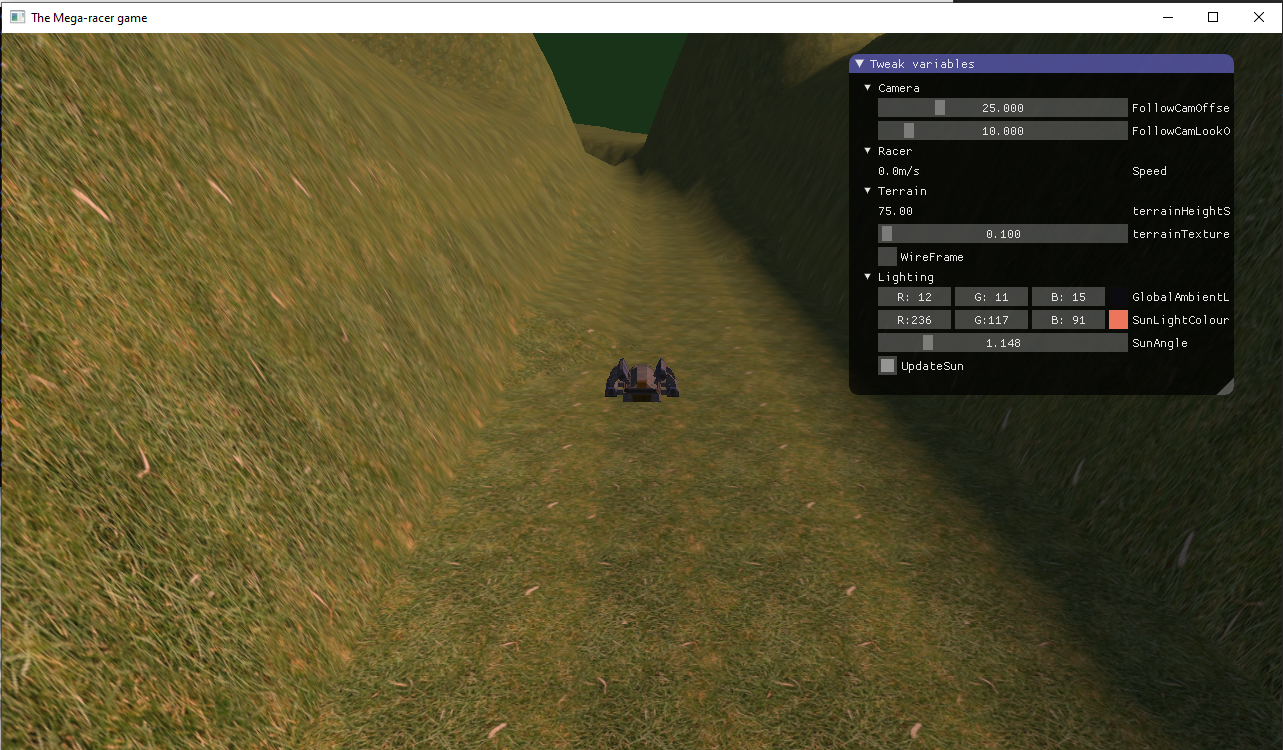
\includegraphics[width=0.49\textwidth, frame]
            {./images/1.5_e_1.PNG}%
        \hfill
        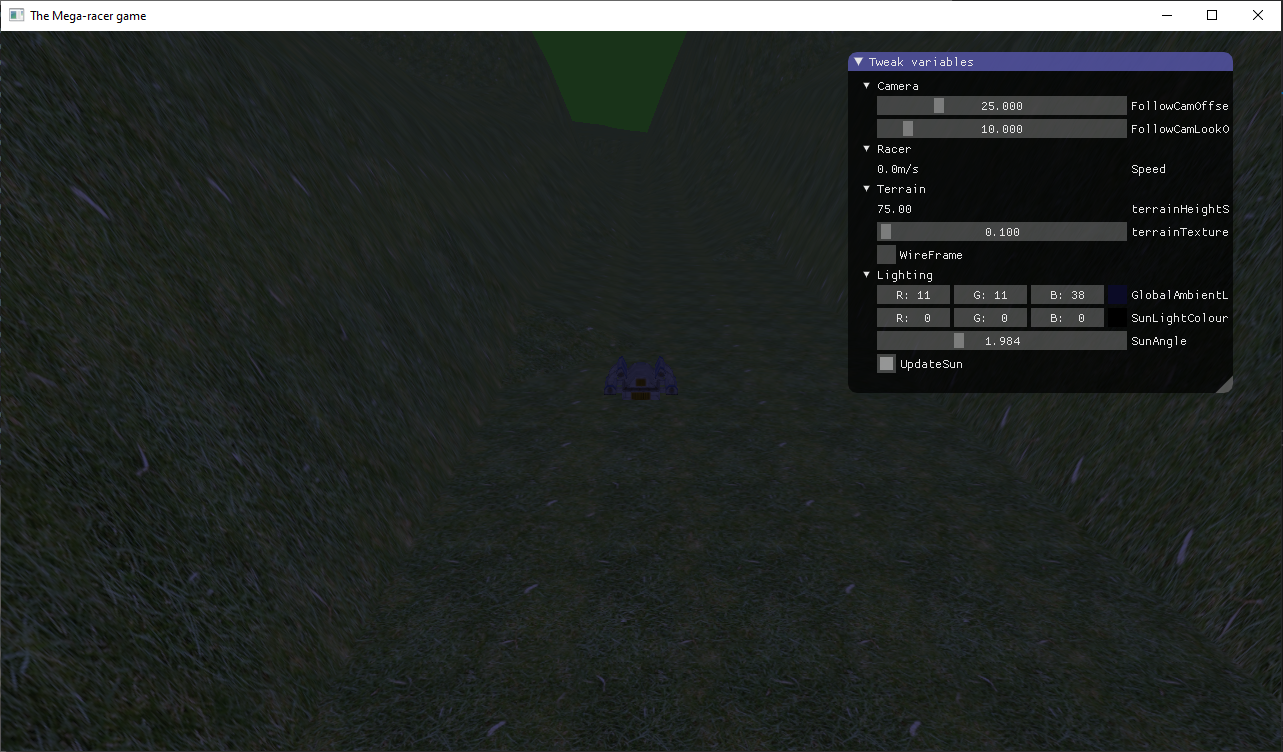
\includegraphics[width=0.49\textwidth, frame]
            {./images/1.5_e_2.PNG}
        }
        
        \caption{1.5 - Step 5}   
    \end{figure}

\textbf{Side notes:}
    \begin{itemize}
        \item As an aside, a slightly more advanced ambient  model, which is sometimes used for outdoor scenes is to have two colours and blend between
        them based on the orientation of the surface, such that things facing straight up get a blue ambient light (from the sky) and down a green tint (to represent grass reflecting light up). We will leave that for now though!
        \item Specular lighting
    \end{itemize}

\subsection{2.1 Improve terrain textures}

\textbf{(1) Set the high texture}
To set the high texture need to use the height and mix with the grass texture. The height is given by the vertex shader, which is the z position of the positionIn or worldSpacePosition variable. The terrainHeightScale is equivalent to Terrain.heightScale which is 75.0 and used as a scale factor to calculate the z coordinates for each vertex.
    \begin{lstlisting}[language=python]
# vertexShader:
v2f_height = positionIn.z
    -> v2f_worldSpacePosition = positionIn 

# render
terrainHeightScale = self.heightScale 
    -> heightScale = 75.0
    \end{lstlisting}

The same steps as the grass texture are followed including declaring a unit, the texture variable, binding the texture, setting the uniform value and loading the texture. However, sampling the texture is slightly different as instead of overriding the materialColour with the highColour, the texture should only appear at set heights and be blended with the grassColour.

\begin{lstlisting}[language=python]
    # terrain.py
    TU_High = 1
    highTexture = None
    
    def render():
        ....
        lu.bindTexture(self.TU_High, self.highTexture)
        lu.setUniform(self.shader, "highTexture", self.TU_High)
    
    def load():
        fragmentShader = 
            ...
            uniform sampler2D highTexture;
    
            void main():
            {   
                ????
            }
        
        self.highTexture = ObjModel.loadTexture("rock 2.png", "data", True)        
        \end{lstlisting}




...... About mix function ....
\begin{lstlisting}[language=python]
def mix(v0, v1, t):
    return v0 * (1.0 - t) + v1 * t
\end{lstlisting}




    \begin{lstlisting}[language=python]

def load():
    fragmentShader = 
        ...   
        void main():
        {   ....
            OR if (v2f_height > 50) {
            if ((v2f_height/terrainHeightScale) > 0.9) {
                vec3 highColour = texture(highTexture, 
                                    v2f_worldSpacePosition.xy 
                                    * terrainTextureXyScale).xyz;
                materialColour = mix(materialColour, 
                                    highColour, 
                                    (v2f_height/terrainHeightScale));
        }       
    \end{lstlisting}


    \begin{figure} [H]
        \centering
        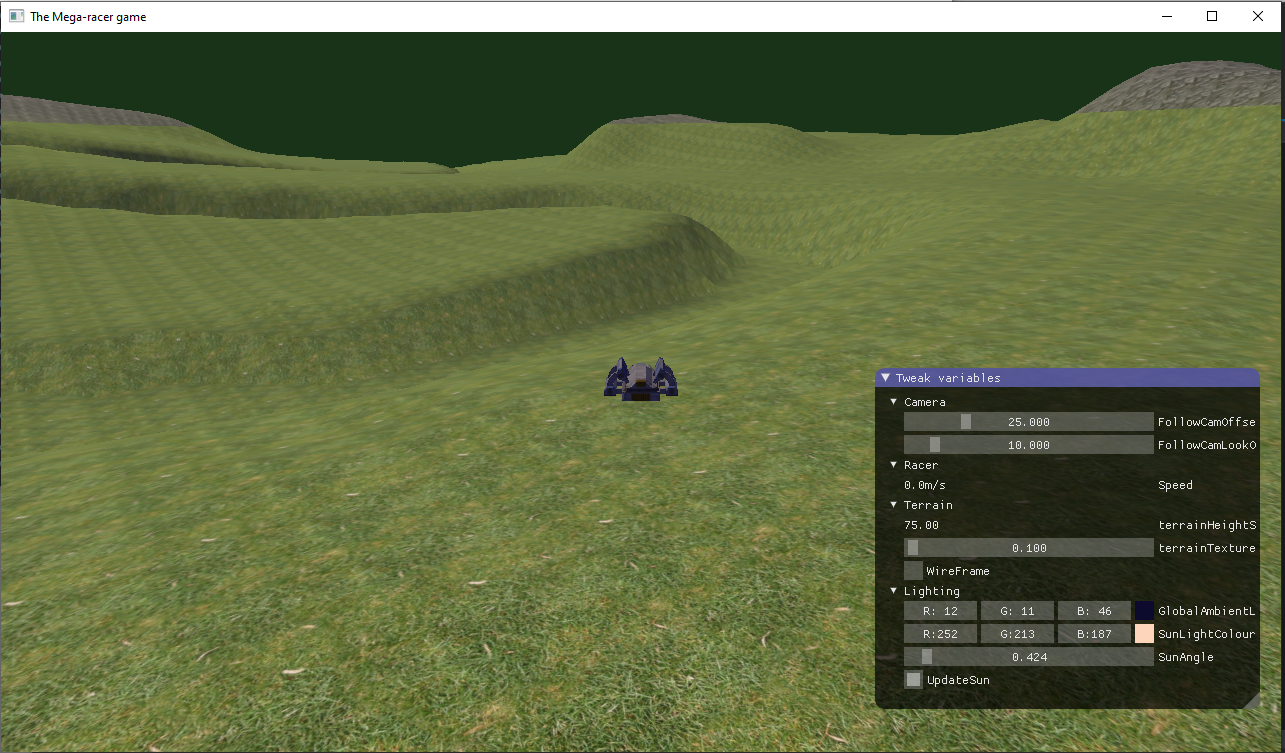
\includegraphics[width=0.8\textwidth, frame]
            {./images/2.1_a.PNG}
        \caption{2.1 - High Texture}   
    \end{figure}


\textbf{(2) Set the steep texture}
First thing is to get the coordinates of the normalised world space. The viewSpacePosition, viewSpaceNormal and worldSpacePosition had already been calculated so I followed the same pattern to get the worldSpaceNormal.

    \begin{lstlisting}
    vertexShader =
        out VertexData
        {
            vec3 v2f_viewSpacePosition;
            vec3 v2f_viewSpaceNormal;
            vec3 v2f_worldSpacePosition;
            vec3 v2f_worldSpaceNormal; // NEW
        }
        void main()
        {
            v2f_viewSpacePosition = (modelToViewTransform * vec4(positionIn, 1.0)).xyz;
            v2f_viewSpaceNormal = modelToViewNormalTransform * normalIn;
            v2f_worldSpacePosition = positionIn;
            v2f_worldSpaceNormal = normalIn; // NEW
        }
    fragmentShader = 
        in VertexData
        {
            vec3 v2f_viewSpacePosition;
            vec3 v2f_viewSpaceNormal;
            vec3 v2f_worldSpacePosition;
            vec3 v2f_worldSpaceNormal; // NEW
        }
    \end{lstlisting}

    Now that the normalised world space is available to use, the slope needs to be calculated and compared to the threshold to determine when to blend the textures.

    \begin{lstlisting}
    # terrain.py
    TU_Steep = 2
    steepTexture = None

    def render():
        ....
        lu.bindTexture(self.TU_Steep, self.steepTexture)
        lu.setUniform(self.shader, "steepTexture", self.TU_Steep)

    def load():
        fragmentShader = """
            ...
            uniform sampler2D steepTexture;

            void main()
            {....
                float slope = dot(v2f_worldSpaceNormal, vec3(v2f_worldSpaceNormal.x, 0.0, v2f_worldSpaceNormal.z));
                if (slope < 0.8) {
                    vec3 steepColour = texture(steepTexture, v2f_worldSpacePosition.xy * terrainTextureXyScale).xyz;
                    materialColour = mix(materialColour, steepColour, (v2f_height/terrainHeightScale));
            } 

        self.steepTexture = ObjModel.loadTexture("rock 5.png", "data", True)
    \end{lstlisting}

    \begin{figure} [H]
        \centering
        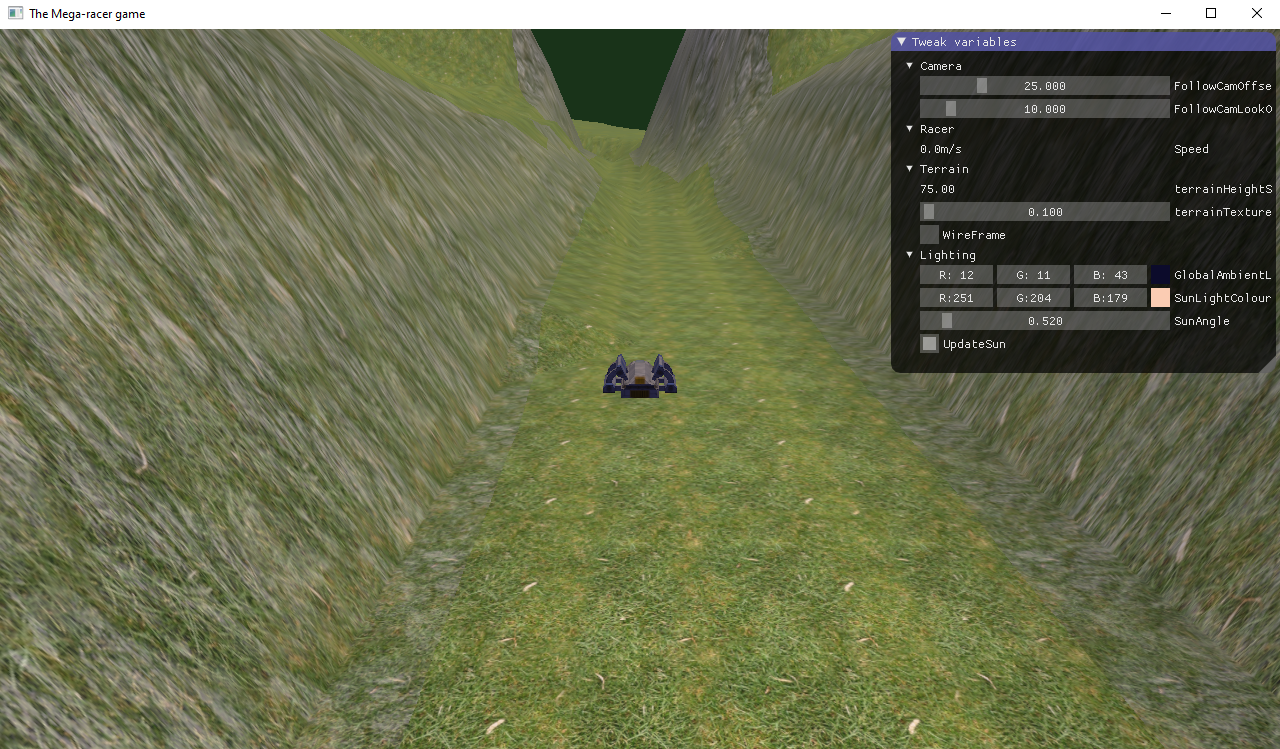
\includegraphics[width=0.8\textwidth, frame]
            {./images/2.1_b.PNG}
        \caption{2.1 - Steep Texture}   
    \end{figure}




\textbf{(3) Add the road}
The same steps for the other textures were then applied to roadTexture and mapTexture, except for the sampling in the main() of fragmentShader as this would be a little different. Also, when using ObjModel.loadTexture since the track image is not a SRGB file, the argument for the srgb parameter is False. 
\begin{lstlisting}
    # terrain.py
    TU_Road = 3
    TU_Map = 4
    roadTexture = None
    mapTexture = None

    def render():
        ....
        lu.bindTexture(self.TU_Road, self.roadTexture)
        lu.bindTexture(self.TU_Map, self.roadMap)
        lu.setUniform(self.shader, "roadTexture", self.TU_Road)
        lu.setUniform(self.shader, "mapTexture", self.TU_Map)

    def load():
        fragmentShader = 
            ...
            uniform sampler2D roadTexture;
            uniform sampler2D mapTexture;

            void main():
            {   ....
                ????
            }
            }
        
        self.roadTexture = ObjModel.loadTexture("paving 5.png", "data", True)
        self.mapTexture = ObjModel.loadTexture("track_01_128.png", "data", False)
\end{lstlisting}


Since the shader doesn't have access to the type of terrain (previously relying on height and slope), the blueChannel needs to be able to be accessed so the shader knows what is considered 'road'. To be able to sample this texture the first step was to get the normalised texture coordinates. This was possible by following the similar steps to the worldSpaceNormal but with the xyNormScale and xyOffset. I knew I needed to use the xyNormScale variable instead of terrainTextureXyScale, but I wasn't sure of the purpose of offset yet. These were the last two declared variables in the vertex shader that hadn't been carried through to the fragment shader despite being declared as uniform in render() at the same time as the Texture XyScale and HeightScale.
\begin{lstlisting}

    # render()      
    xyNormScale = 1.0 / (vec2(self.imageWidth, self.imageHeight) * self.xyScale);
    lu.setUniform(self.shader, "xyNormScale", xyNormScale);
    xyOffset = -(vec2(self.imageWidth, self.imageHeight) + vec2(1.0)) * self.xyScale / 2.0;
    lu.setUniform(self.shader, "xyOffset", xyOffset);

    --> 

    # load()
    vertexShader =
        out VertexData
        {
            vec2 v2f_xyNormScale;
            vec2 v2f_xyOffset;
        }
        void main()
        {
            v2f_xyNormScale = xyNormScale;
            v2f_xyOffset = xyOffset;
        }
    fragmentShader = 
        in VertexData
        {
            vec2 v2f_xyNormScale;
            vec2 v2f_xyOffset;
        }
    \end{lstlisting}

When working on this section, it was often difficult to determine the problem, as unless the texture was declared, bound and loaded properly in the shader nothing would display. The below code is the first iteration that provided 'working' shading. The blueChannel variable followed that of the other textures, though instead of multiplying the worldSpacePosition.xy by the terrainTextureXyScale it was multiplied by the xyNormScale variable and only the z coordinate needed to be stored. The threshold of 0.9 was chosen as this produced the most accurate result. 
    \begin{lstlisting}
    # terrain.py       
    def load():
        fragmentShader =                 
            void main():
            {   ....
            float blueChannel = texture(mapTexture, (v2f_worldSpacePosition.xy) * v2f_xyNormScale).z;
            if (blueChannel >= 0.9) {
                vec3 roadColour = texture(roadTexture, v2f_worldSpacePosition.xy * terrainTextureXyScale).xyz;
                materialColour =  mix(materialColour, roadColour, (v2f_height/terrainHeightScale));
                }
            }
    \end{lstlisting} 
    
When I finally did get the shader working to a point that it would display it was clear that there were still a couple of issues to resolve.

\begin{figure} [H]
    \centering
    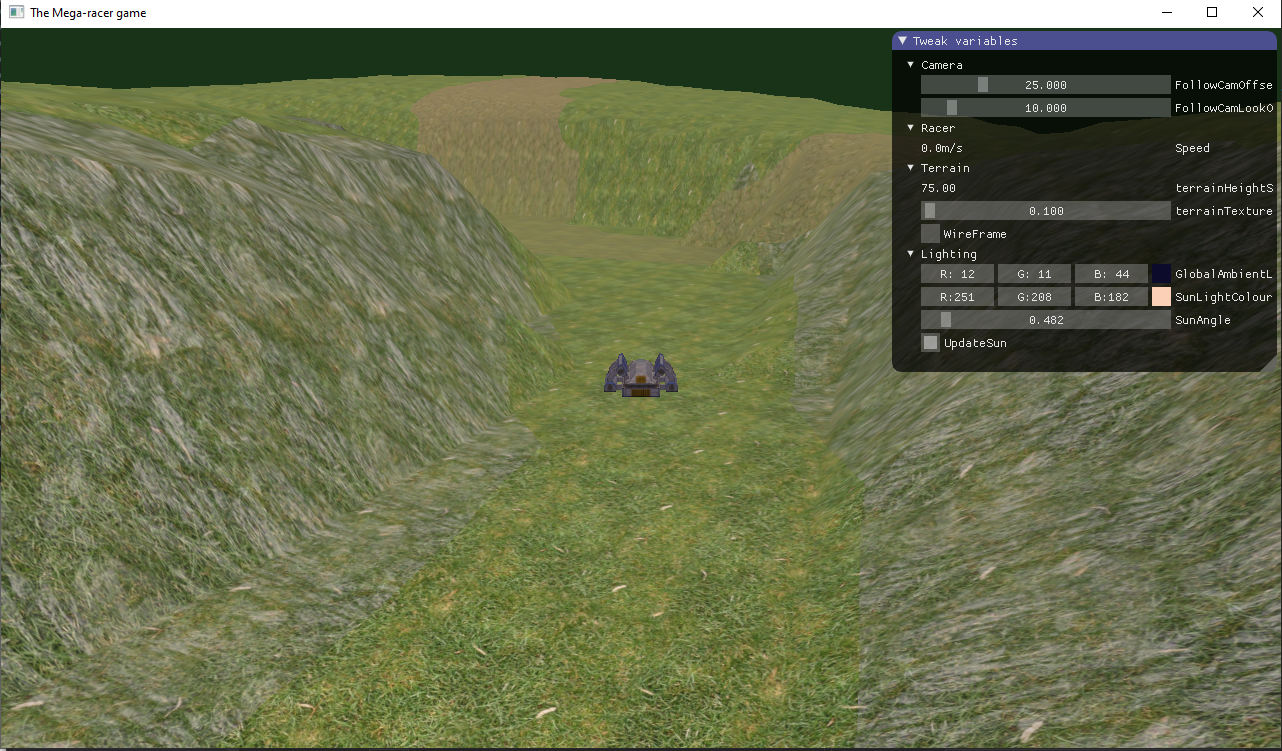
\includegraphics[width=0.8\textwidth, frame]
        {./images/2.1_c_1.PNG}
    \caption{2.1 - Road Texture (Mixed \& No Offset)}   
\end{figure}

\begin{enumerate}
    \item The grass texture was overtaking the blend of the pavement. This is because I mixed the roadColour with the grassColour as previously done, instead I did the same as that for the grassColour and declared the materialColour of the road to be only roadColour
    \item The road was not in the position it needed to be and was instead on the hill. This was another simple fixing by subtracting the xyOffset variable from the worldSpacePosition. After discovering this fixed the coordinates of the road I also tried mixing the road and grass colours again but the sample problem occurred.
\end{enumerate}

\begin{figure} [H]
        \makebox[\textwidth]{%
        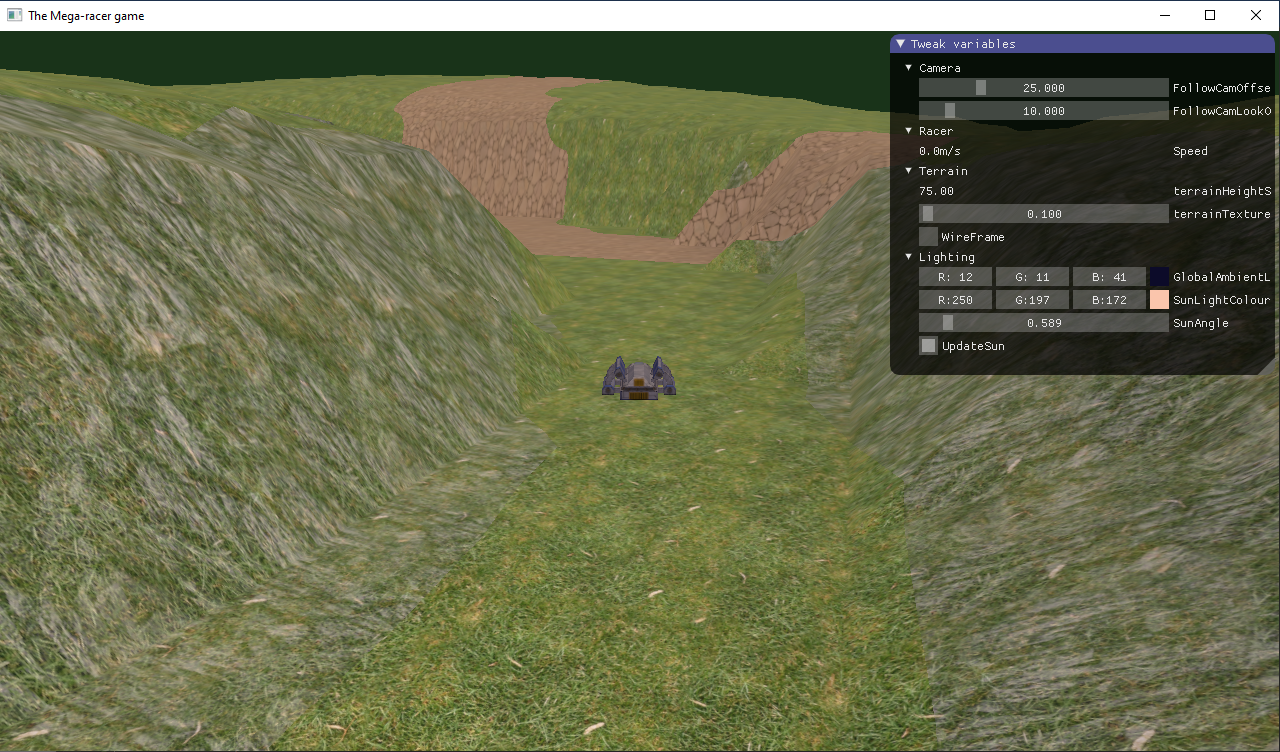
\includegraphics[width=0.49\textwidth, frame]
            {./images/2.1_c_2.PNG}%
        \hfill
        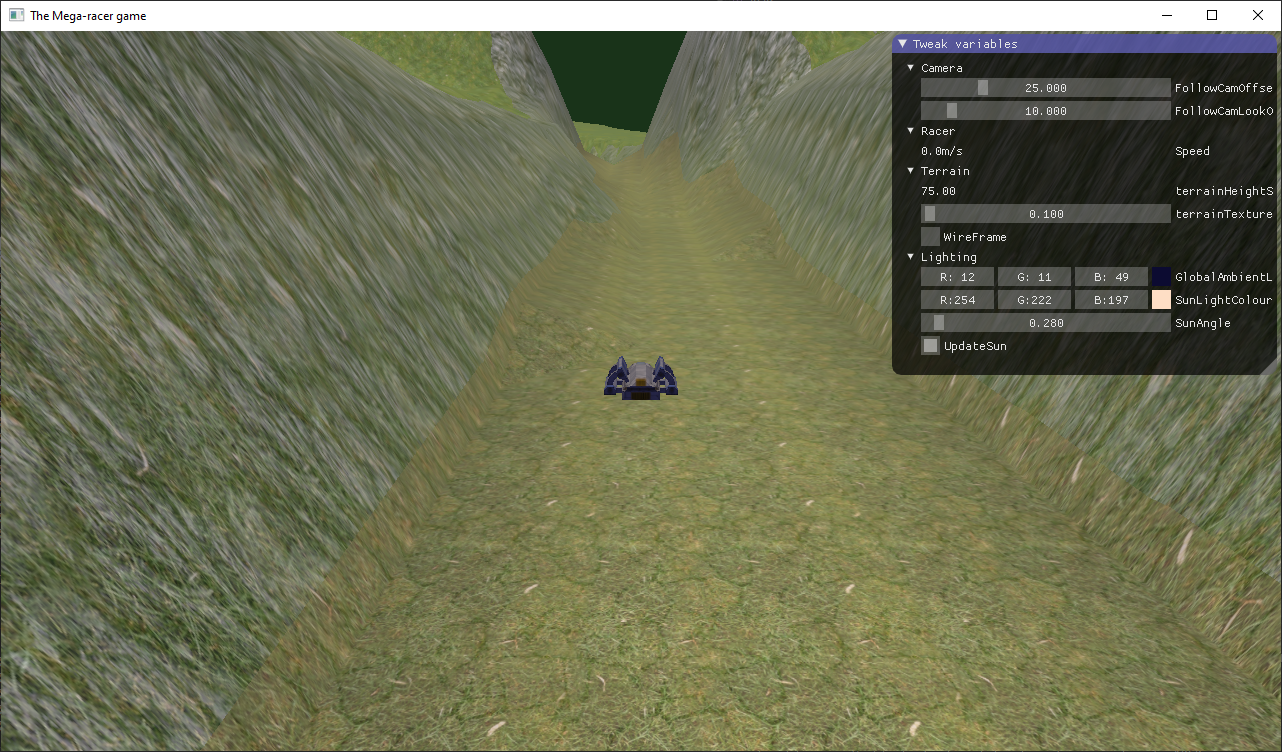
\includegraphics[width=0.49\textwidth, frame]
            {./images/2.1_c_3.PNG}        
        }        
        \caption{2.1 - Road Texture (Not Mixed \& No offset / Mixed \& Offset)}   
\end{figure}


After making these changes, the paving was successfully sampled and loading correctly onto the correct coordinates for the road according to the blue channel of the track.

    \begin{lstlisting}
    # terrain.py       
    float blueChannel = texture(mapTexture, (v2f_worldSpacePosition.xy - v2f_xyOffset) * v2f_xyNormScale).z;
    if (blueChannel >= 0.9) {
        vec3 roadColour = texture(roadTexture, v2f_worldSpacePosition.xy * terrainTextureXyScale).xyz;
            materialColour = roadColour;
    }
    \end{lstlisting} 

    \begin{figure} [H]
        \centering
        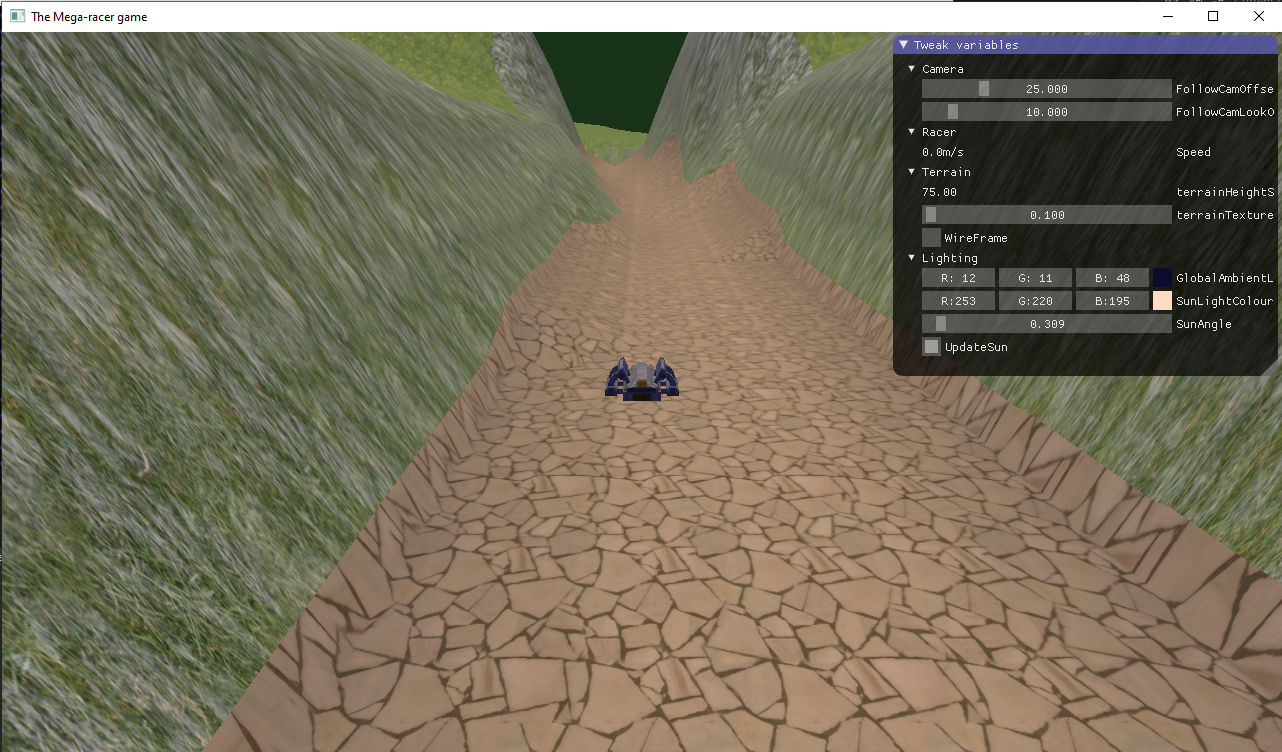
\includegraphics[width=0.8\textwidth, frame]
            {./images/2.1_c_final.PNG}
        \caption{2.1 - Road Texture}   
    \end{figure}





\end{document}